%%%%%%%%%%%%%%%%%%%%%%%%%%%%%%%%%%%%%%%%%%%%%%%%%%%%%%%%%%%%%%%%%%
% Artigo segundo as normais mais atualizadas da ABNT
% Baseado no template de A. J. Bühler e Berg Dantas 
%%%%%%%%%%%%%%%%%%%%%%%%%%%%%%%%%%%%%%%%%%%%%%%%%%%%%%%%%%%%%%%%%%
\documentclass[article,12pt,oneside,a4paper,english,brazil,sumario=tradicional]{abntex2}		

% --- PACOTES ---
\usepackage[T1]{fontenc}                % Selecao de codigos de fonte.
\usepackage[utf8]{inputenc}             % Codificacao do documento
\usepackage{times}                      % Usa a fonte Times New Roman
\usepackage{indentfirst}                % Indenta o primeiro parágrafo de cada seção.
\usepackage{color}                      % Controle das cores
\usepackage{graphicx, subcaption}       % Inclusão de gráficos e subfiguras
\usepackage{microtype}                  % Para melhorias de justificação
\usepackage[abnt-emphasize=bf,abnt-and-type=e,alf,doi=true]{abntex2cite}% Citações ABNT (estilo autor-data)
\usepackage{url}
\usepackage{mathptmx}
\usepackage{amsmath}
\usepackage{hyperref} 
\usepackage{multirow}				    % Permite maior formatação de tabelas
\usepackage{booktabs}                   % Para tabelas com melhor visual
\usepackage{tikz}                       % Para desenhar diagramas
\usetikzlibrary{calc, positioning, arrows.meta} % Bibliotecas do TikZ

% --- CONFIGURACOES DE PACOTES ---
\definecolor{blue}{RGB}{41,5,195}
\hypersetup{
	colorlinks=true,
	linkcolor=blue,
	citecolor=blue,
	filecolor=magenta,
	urlcolor=blue,
}

% --- CONFIGURACOES DO DOCUMENTO ---
\graphicspath{{./Figuras/}}             % Pasta para as figuras
\setsecheadstyle{\bfseries \normalsize \uppercase}
\setsubsecheadstyle{\normalsize \uppercase}
\setsubsubsecheadstyle{\bfseries \normalsize}
\setlrmarginsandblock{3cm}{2cm}{*}      % Margens esquerda-direita
\setulmarginsandblock{3cm}{2cm}{*}      % Margens cima-baixo
\checkandfixthelayout
\setlength{\parindent}{1.25cm}           % Tamanho do parágrafo
\OnehalfSpacing                         % Espaçamento de 1,5
\setlength{\ABNTEXcitacaorecuo}{4cm}     % Recuo para citação direta com mais de 3 linhas

\begin{document}
\selectlanguage{brazil} % Seleciona o idioma do documento
\frenchspacing          % Retira espaço extra obsoleto entre as frases.
				
% --- CABEÇALHO ---
\begin{center}
\Large{\textbf{Estudo reológico de suspensões de caulim e validação de \\ um reômetro capilar de baixo custo}} \vspace{12pt}
	
	\small%{Mestrado Profissional em Tecnologia e Engenharia de Materiais - IFRS}
	
	\vspace{12pt}
	
    % Autores e Afiliações conforme Anexo I do Edital
    \textbf{Bruno Kenji Nishitani Egami¹}, \textbf{Prof. Dr. André Zimmer²}, \textbf{Profª. Drª. Daniela Lupinacci Villanova¹*}
    
    \vspace{12pt} % Espaçamento entre autores e afiliações
    
    \footnotesize{
    *Orientadora \\
    ¹Instituto Federal de Educação, Ciência e Tecnologia do Rio Grande do Sul (IFRS) - Campus Farroupilha \\
    ²Instituto Federal de Educação, Ciência e Tecnologia do Rio Grande do Sul (IFRS) - Campus Feliz
    }
\end{center}

\hrule
\SingleSpacing
\noindent


\textual
\pagestyle{simple}
\aliaspagestyle{chapter}{simple}
\thispagestyle{empty}

% --- SEÇÕES DO ARTIGO ---
\noindent
\\ \textbf{Palavras-chave}: Reologia, Suspensões Cerâmicas, Reômetro Capilar. 

\section{Introdução}
\label{sec:introducao}
\normalsize
A ciência e engenharia de materiais estabelecem que as propriedades de um material são uma consequência de sua estrutura e de como ele é processado. Nos materiais cerâmicos, essa relação é particularmente importante. O sucesso de processos de fabricação via úmida, como colagem, extrusão e atomização, depende diretamente do controle das propriedades de fluxo da suspensão, o que constitui o campo de estudo da reologia. A reologia surge, portanto, como uma ferramenta essencial para o desenvolvimento de suspensões que sejam, ao mesmo tempo, concentradas e fluidas, um requisito para obter produtos finais densos e com boa resistência mecânica \citeonline{reed1995}.

Recentemente, a manufatura aditiva (AM), ou impressão 3D, tem emergido como uma tecnologia versátil para a fabricação de cerâmicas. Dentre as técnicas de AM, destaca-se a \textit{Direct Ink Writing} (DIW), também conhecida como \textit{Robocasting}, que consiste na extrusão de pastas viscosas camada por camada para construir um objeto tridimensional \citeonline{dewitte2022}. Este método se caracteriza pelo uso de pastas com alta concentração de sólidos e comportamento pseudoplástico, permitindo a consolidação das camadas depositadas \citeonline{shahzad2021}. A impressão 3D cerâmica oferece elevada liberdade geométrica, possibilitando a criação de estruturas complexas que seriam inviáveis por métodos tradicionais \citeonline{oliveira2024}.

O sucesso da impressão 3D por DIW depende de um controle reológico rigoroso. Conforme destacado por \citeonline{pires2023}, as pastas devem atender a requisitos específicos, como comportamento pseudoplástico que permita o escoamento pelo bico e rápida recuperação da viscosidade para suportar as camadas subsequentes sem deformar (\textit{buildability}). Nesse contexto, a caracterização reológica precisa do material base é um passo fundamental.

Este estudo, desenvolvido no âmbito do Mestrado Profissional em Tecnologia e Engenharia de Materiais do IFRS, aborda um problema de pesquisa central: a caracterização reológica precisa, fundamental para o avanço de tecnologias como a impressão 3D cerâmica, frequentemente depende de equipamentos comerciais de alto custo, o que limita o acesso à pesquisa e ao desenvolvimento de novos materiais. Para enfrentar essa barreira, o trabalho estabelece um duplo objetivo: primeiramente, caracterizar o comportamento de suspensões de caulim-água, servindo como uma base de conhecimento; e, em paralelo, desenvolver e validar um reômetro capilar de baixo custo como uma ferramenta alternativa e acessível para essa análise, posicionando-se como uma etapa fundamental para futuras aplicações em manufatura aditiva.

\section{Metodologia}
\label{sec:experimental}

\subsection{Materiais e Métodos}
\subsubsection{Materiais e Preparação das Amostras}
O caulim industrial utilizado nos ensaios foi adquirido da empresa BRX Minérios (São Caetano do Sul/SP). As suspensões foram preparadas inserindo-se as massas pré-determinadas de caulim e água destilada em um saco plástico. A mistura foi então homogeneizada por agitação manual até a obtenção de uma pasta uniforme. Este método também facilitou a alimentação dos reômetros, cortando-se uma extremidade do saco para transferir a pasta. As concentrações de caulim e água, em percentuais de massa, são detalhadas na Tabela \ref{tab:concentracoes}.

\begin{table}[htbp]
\centering
\caption{Formulações das suspensões de caulim analisadas.}
\label{tab:concentracoes}
\begin{tabular}{@{}ccc@{}}
\toprule
\textbf{Amostra} & \textbf{\% de Caulim (Sólidos)} & \textbf{\% de Água} \\ \midrule
A & 75,0\% & 25,0\% \\
B & 70,0\% & 30,0\% \\
C & 67,5\% & 32,5\% \\
D & 65,0\% & 35,0\% \\
E & 62,5\% & 37,5\% \\
F & 60,0\% & 40,0\% \\ \bottomrule
\end{tabular}
\end{table}

Amostras com teor de sólidos superior a 67,5\% (A e B) foram descartadas por apresentarem baixa plasticidade, resultando em uma massa seca e sem coesão ("farofa"), inviável para os ensaios.

\subsubsection{Equipamentos de Análise Reológica}
Foram utilizados dois equipamentos para a caracterização reológica das suspensões Figura \ref{fig:reometros}. Um reômetro Anton Paar, modelo MCR 102, com geometria de pratos paralelos (25 mm de diâmetro) foi utilizado como equipamento de referência e serviu de base para comparação com o reômetro capilar de baixo custo desenvolvido.  

\begin{figure}[h!]
    \centering
    \begin{subfigure}[b]{0.35\textwidth}
        \centering
        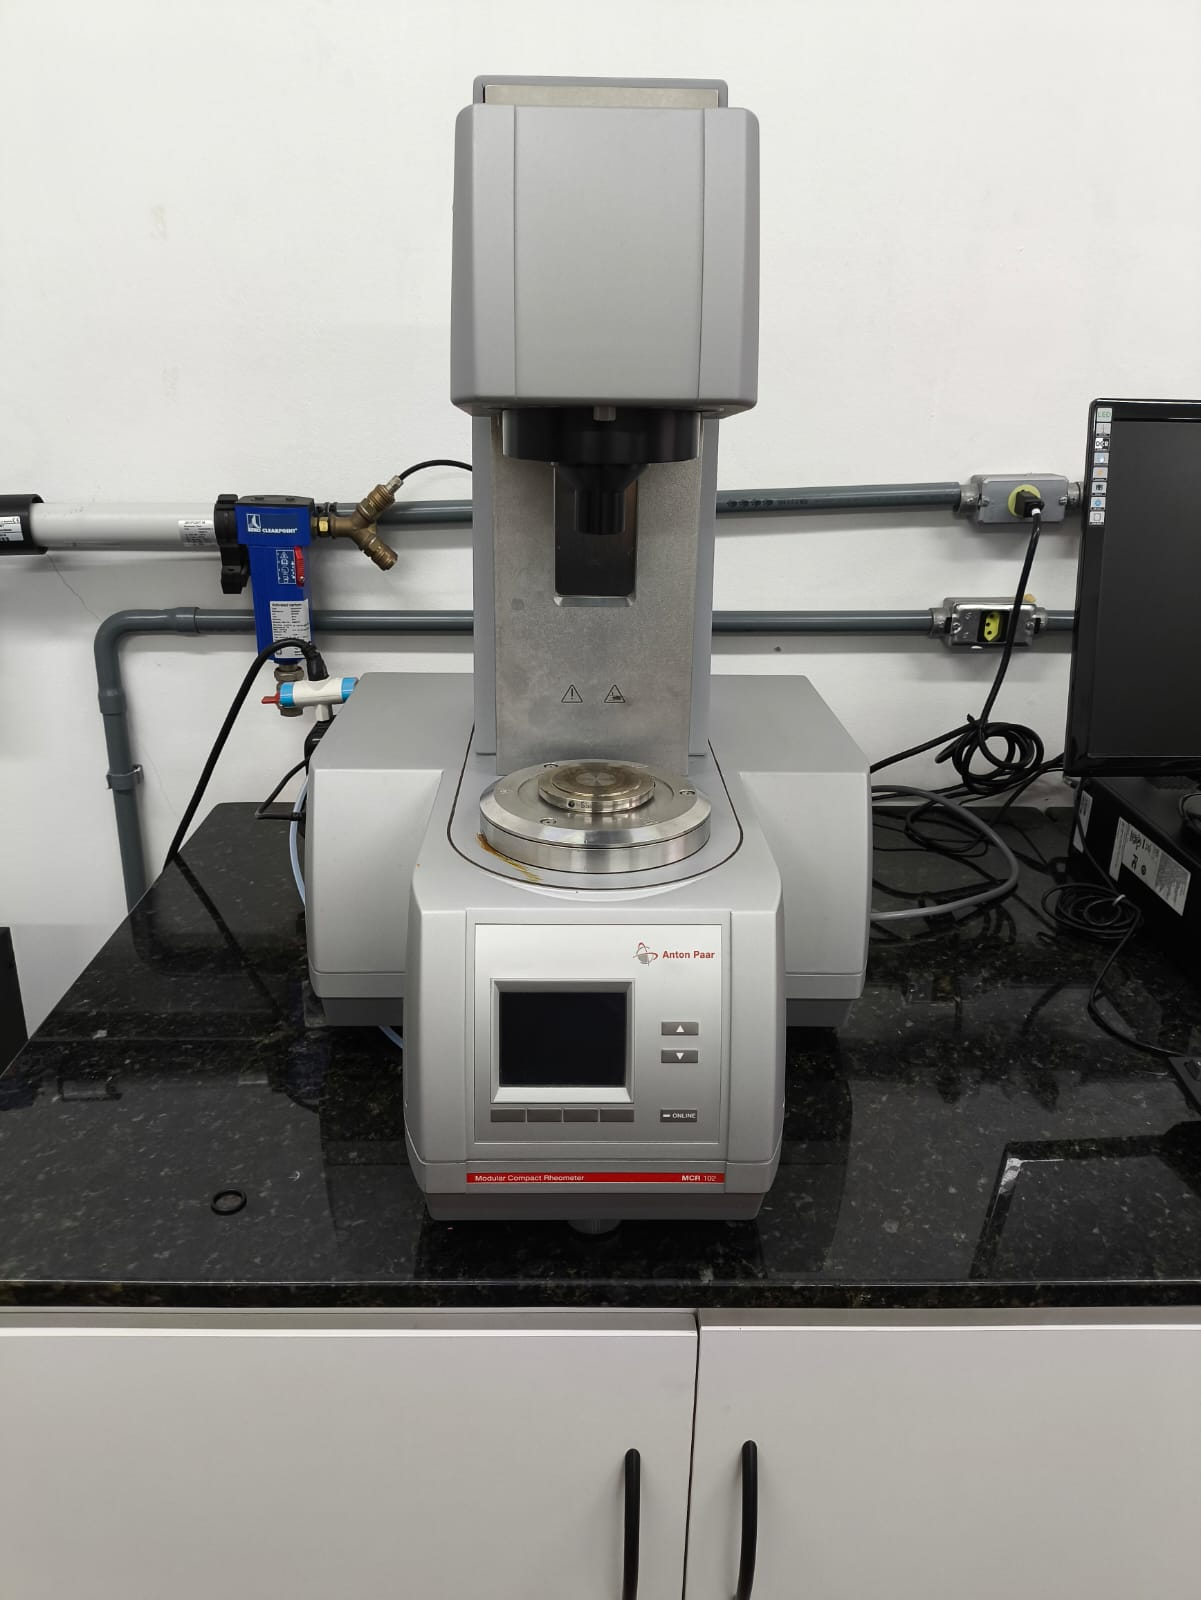
\includegraphics[width=\textwidth]{reometro_rotacional.jpeg}
        \caption{Reômetro rotacional comercial.}
        \label{fig:reometro_comercial}
    \end{subfigure}
    \hfill
    \begin{subfigure}[b]{0.35\textwidth}
        \centering
        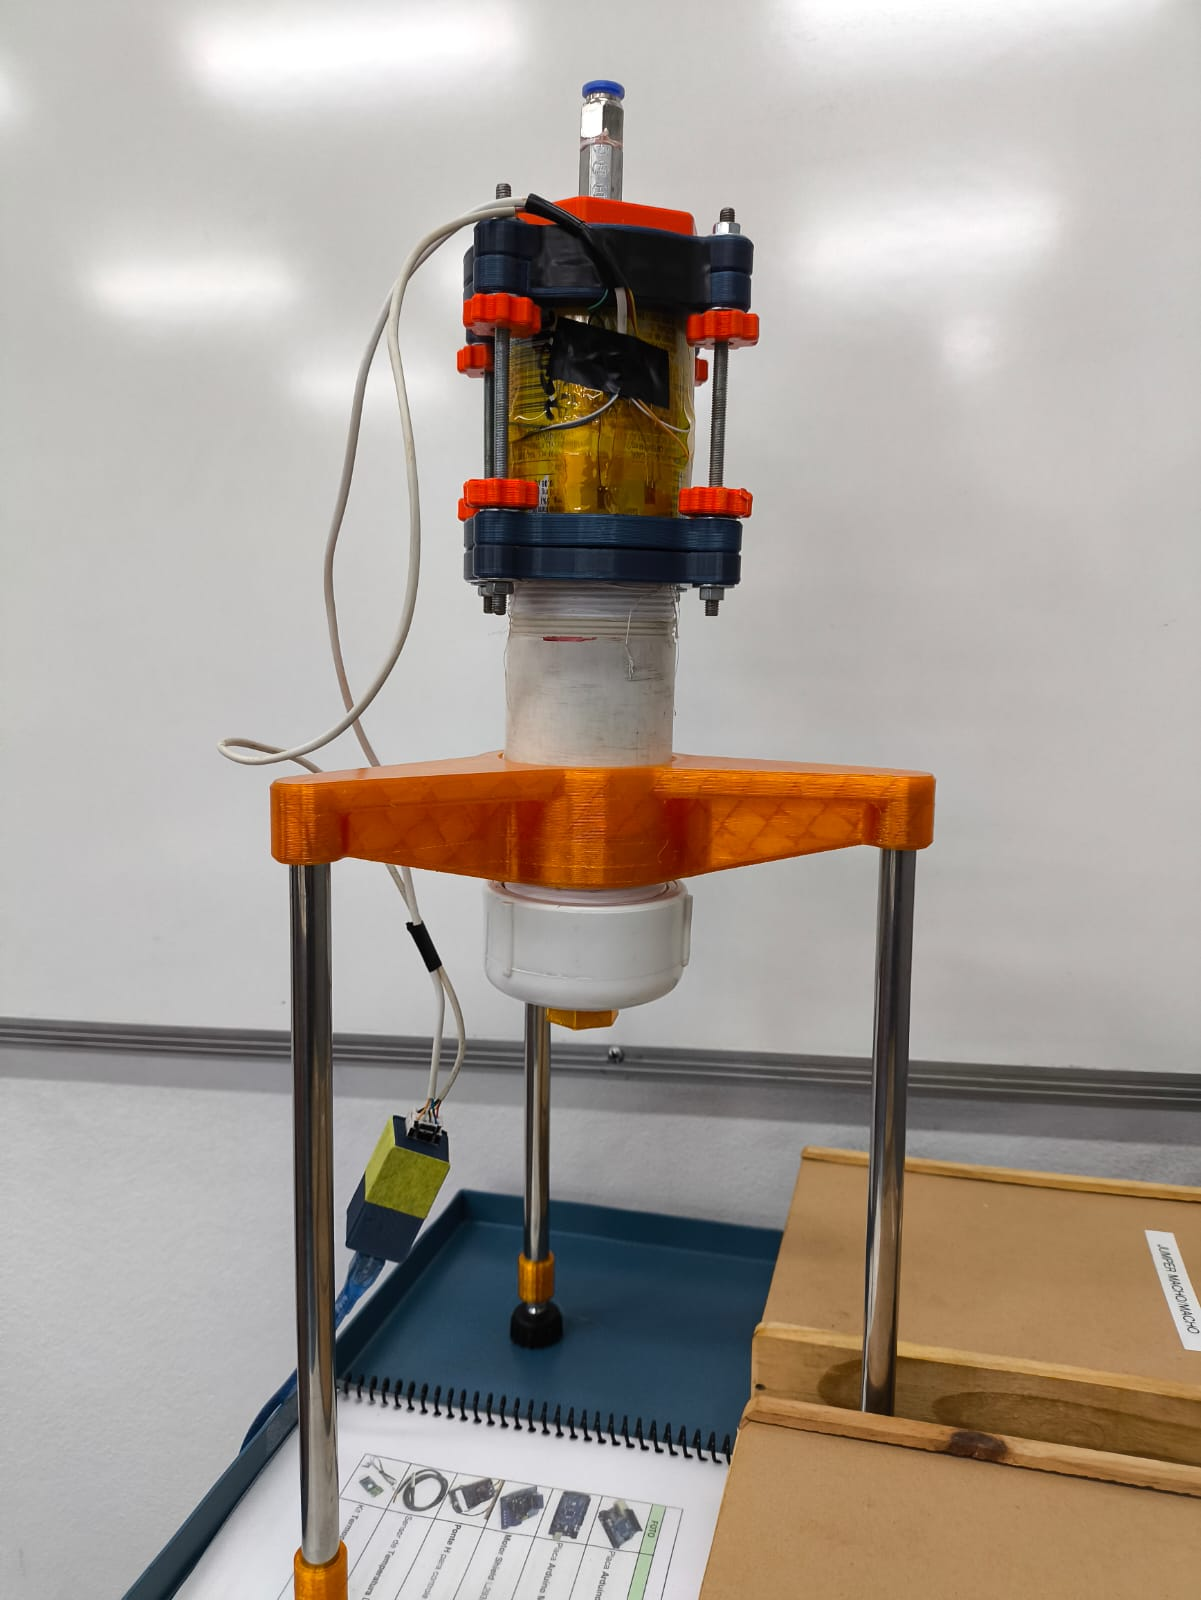
\includegraphics[width=\textwidth]{reometro_capilar.jpeg}
        \caption{Reômetro capilar de baixo custo.}
        \label{fig:reometro_diy}
    \end{subfigure}
    \caption{Equipamentos utilizados para a análise reológica.}
    \label{fig:reometros}
\end{figure}

 

\subsection{Desenvolvimento do Reômetro Capilar de Baixo Custo}
\label{subsubsec:reometro-capilar}
O reômetro capilar de baixo custo foi desenvolvido com foco em replicabilidade e precisão para operar em taxas de cisalhamento mais elevadas. Sua estrutura principal utiliza um corpo de PVC, pistão e capilares fabricados por impressão 3D. O sistema de medição de pressão é composto por uma célula de carga customizada (com \textit{strain gauges} e um módulo amplificador HX711), gerenciada por um microcontrolador Arduino. O controle do ensaio e a análise de dados são automatizados por um conjunto de scripts em Python, que gerenciam a aquisição de dados, realizam a calibração do sensor, calculam os parâmetros reológicos com as devidas correções, ajustam os dados a modelos matemáticos e geram relatórios e gráficos comparativos. O esquema de funcionamento do sistema está ilustrado na Figura \ref{fig:esquema_reometro}.

\begin{figure}[htbp]
\centering
\resizebox{0.95\textwidth}{!}{%
\begin{tikzpicture}[node distance=2cm, auto]
    % Carregar bibliotecas
    \usetikzlibrary{calc, positioning}

    % Definindo os estilos
    \tikzstyle{block} = [rectangle, draw, fill=blue!20, text width=8em, text centered, rounded corners, minimum height=3em]
    \tikzstyle{instrument} = [circle, draw, fill=orange!30, text centered, minimum size=5em, align=center]
    \tikzstyle{data_block} = [rectangle, draw, fill=purple!20, text width=8em, text centered, rounded corners, minimum height=3em]
    \tikzstyle{line} = [draw, thick, -{Stealth[length=3mm]}]
    \tikzstyle{data_line} = [draw, thick, dashed, color=green!60!black, -{Stealth[length=3mm]}]
    \tikzstyle{manual_line} = [draw, thick, dotted, color=red!80!black, -{Stealth[length=3mm]}]

    % Posicionando os nós (componentes) na horizontal
    \node [block] (compressor) {Compressor};
    \node [block, right=1.5cm of compressor] (regulator) {Registro Regulador de Pressão};
    \node [instrument, right=1.5cm of regulator] (manometer) {Manômetro};
    \node [block, right=1.5cm of manometer] (valve) {Válvula de Bloqueio};
    \node [block, right=1.5cm of valve] (rheometer) {Corpo do Reômetro};

    % Ponto de tomada de pressão (entre a válvula e o reômetro)
    \coordinate (tap_point) at ($(valve.east)!0.5!(rheometer.west)$);

    % Linha de Dados (abaixo da linha principal)
    \node [instrument, below=2cm of tap_point] (transducer) {Strain \\ Gauges};
    \node [data_block, left=2cm of transducer] (arduino) {Arduino};
    \node [data_block, left=2cm of arduino] (computer) {Computador (Python)};
    
    % Balança para medição de massa, posicionada mais abaixo do reômetro para evitar sobreposição
    \node [data_block, below=3.5cm of rheometer] (balance) {Balança};

    % Desenhando as linhas de conexão
    % Linha Pneumática Principal
    \path [line] (compressor) -- (regulator);
    \path [line] (regulator) -- (manometer);
    \path [line] (manometer) -- (valve);
    \path [line] (valve) -- (rheometer);
    
    % Linha de Pressão para o Transdutor
    \path [line] (tap_point) -- (transducer);
    
    % Linha de Dados Automática
    \path [data_line] (transducer) -- (arduino);
    \path [data_line] (arduino) -- (computer);
    
    % Fluxo de material para a balança (agora como coleta manual)
    \path [manual_line] (rheometer) -- (balance);
    
    % Linha de Dados Manual em "L"
    \path [manual_line] (balance) -| (computer.south);
\end{tikzpicture}
}
\caption{Esquema de funcionamento do reômetro capilar, mostrando a linha pneumática (sólida), a linha de aquisição de dados automática (tracejada) e as linhas de coleta e entrada de dados manual (pontilhada).}
\label{fig:esquema_reometro}
\end{figure}

 A documentação completa do projeto, incluindo diagramas, códigos e modelos 3D, está disponível em \citeonline{egami2025}.


\subsubsection{Cálculos Reológicos do Reômetro Capilar}
\label{subsubsec:calculos}

A análise reológica busca descrever a relação entre a tensão de cisalhamento ($\tau$), a taxa de cisalhamento ($\dot{\gamma}$) e a viscosidade ($\eta = \tau / \dot{\gamma}$). Em um reômetro capilar, estes parâmetros são obtidos indiretamente a partir de grandezas experimentais: a pressão de extrusão ($P$), a massa de material extrudado ($m$) em um determinado tempo ($t$), e as dimensões do capilar (raio $R$ e comprimento $L$).

O primeiro parâmetro, a \textbf{tensão de cisalhamento na parede} ($\tau_w$), é derivado de um balanço de forças no escoamento dentro do capilar, onde a força gerada pela pressão é equilibrada pela força de atrito viscoso na parede, conforme a equação de \citeonline{barnes1989}:
\begin{equation}
    \tau_w = \frac{P \cdot R}{2 \cdot L}
\end{equation}

O segundo parâmetro é a \textbf{taxa de cisalhamento aparente na parede} ($\dot{\gamma}_{aw}$), calculada a partir da vazão volumétrica ($Q$). O termo \textit{aparente} é utilizado porque sua derivação pressupõe um perfil de velocidade parabólico, que é estritamente válido apenas para fluidos Newtonianos \citeonline{reed1995}:
\begin{equation}
    \dot{\gamma}_{aw} = \frac{4 \cdot Q}{\pi \cdot R^3}
\end{equation}

Como as suspensões cerâmicas são fluidos não-Newtonianos (pseudoplásticos), seu perfil de velocidade é mais achatado, resultando em uma taxa de cisalhamento real na parede superior à aparente. Para corrigir essa distorção, aplica-se a \textbf{correção de Weissenberg-Rabinowitsch}, que converte o valor aparente ($\dot{\gamma}_{aw}$) no valor verdadeiro ($\dot{\gamma}_w$), conforme a equação de \citeonline{barnes1989}:
\begin{equation}
    \dot{\gamma}_w = \frac{\dot{\gamma}_{aw}}{4} \left( 3 + \frac{d(\ln \dot{\gamma}_{aw})}{d(\ln \tau_w)} \right)
\end{equation}

O termo diferencial na equação representa o inverso da inclinação da curva de fluxo em um gráfico log-log e é calculado numericamente a partir dos dados experimentais. Outras correções, como a de Bagley (perdas de pressão na entrada) e Mooney (deslizamento na parede), embora relevantes \citeonline{barnes1989} e previstas no modelamento dos scripts, não foram aplicadas no escopo deste trabalho.

\subsubsection{Procedimento Experimental}
Os ensaios no reômetro capilar foram realizados utilizando-se um capilar com 2 mm de diâmetro e 30 mm de comprimento. Foram analisadas as amostras com 35\%, 37,5\% e 40\% de água (correspondentes às Amostras D, E e F, com 65\%, 62,5\% e 60\% de sólidos, respectivamente). Não foi possível realizar o ensaio nas amostras com teor de água inferiores a 35\% (Amostras C, B e A) em razão da limitação de pressão do conjunto bem como da baixa plasticidade das formulações. A alta concentração de sólidos dessas amostras demanda uma tensão de cisalhamento para o escoamento mais elevada do que o equipamento consegue desenvolver.

Para este estudo, a correção de Weissenberg-Rabinowitsch foi aplicada para converter a taxa de cisalhamento aparente em seu valor verdadeiro, garantindo maior precisão na análise do comportamento do fluido. No entanto, as correções de \textbf{Bagley} e \textbf{Mooney} não foram realizadas, sendo esta uma simplificação adotada para o escopo deste trabalho. A ausência das correções pode introduzir um desvio nos valores absolutos de tensão e viscosidade, mas não invalida a comparação das tendências de comportamento entre os equipamentos.


\section{Resultados e Discussão}
Os resultados comparativos dos ensaios reológicos são apresentados na Figura \ref{fig:resultados_comparativos}.

\begin{figure}[htbp]
    \centering
    \begin{subfigure}[b]{0.49\textwidth}
        \centering
        \includegraphics[width=\textwidth]{Curvas-fluxo_log.png}
        \caption{Curvas de fluxo.}
        \label{fig:fluxo_sub}
    \end{subfigure}
    \hfill % Adiciona um espaço flexível entre as subfiguras
    \begin{subfigure}[b]{0.49\textwidth}
        \centering
        \includegraphics[width=\textwidth]{Curvas-viscosidade_log.png}
        \caption{Curvas de viscosidade.}
        \label{fig:viscosidade_sub}
    \end{subfigure}
    \caption{Resultados reológicos comparativos obtidos no reômetro comercial (MCR102) e no reômetro capilar de baixo custo. Em (a), as curvas de Tensão de Cisalhamento vs. Taxa de Cisalhamento. Em (b), as curvas de viscosidade aparente vs. Taxa de Cisalhamento.}
    \label{fig:resultados_comparativos}
\end{figure}

A análise dos gráficos revela pontos relevantes. Primeiramente, para todas as amostras e em ambos os equipamentos, observa-se um comportamento não-newtoniano do tipo pseudoplástico (\textit{shear-thinning}), onde a viscosidade aparente diminui com o aumento da taxa de cisalhamento. Este é o comportamento característico para suspensões de caulim, conforme documentado na literatura \citeonline{wang2019, castro2016, araujo2008}.

O principal resultado da análise é a validação do reômetro capilar. Ao comparar os dados da amostra de 60\% de caulim (Amostra F) obtidos no MCR102 (círculos roxos) e no reômetro capilar (losangos amarelos), nota-se uma boa concordância na faixa de sobreposição das taxas de cisalhamento. As curvas de fluxo e de viscosidade de ambos os equipamentos apresentam grande proximidade, o que confere confiabilidade aos dados gerados pelo dispositivo de baixo custo, especialmente em taxas de cisalhamento mais altas (acima de 100 $s^{-1}$), onde reômetros capilares são tipicamente mais eficazes.

A Tabela \ref{tab:parametros_reologicos} resume os parâmetros do modelo de Herschel-Bulkley, ajustados a partir dos dados obtidos com o reômetro de baixo custo para as três concentrações analisadas.

\begin{table}[h!]
\centering
\caption{Parâmetros reológicos do modelo de Herschel-Bulkley para as amostras analisadas no reômetro capilar de baixo custo.}
\label{tab:parametros_reologicos}
\begin{tabular}{@{}ccccc@{}}
\toprule
\textbf{Amostra} & \textbf{\% Sólidos} & \textbf{$\tau_0$ (Pa)} & \textbf{K (Pa$\cdot$s$^n$)} & \textbf{n (-)} \\ \midrule
F & 60,0\% & $\approx$ 0 & 77,58 & 0,22 \\
E & 62,5\% & 6,31 & 103,90 & 0,19 \\
D & 65,0\% & 451,35 & 0,09 & 1,02 \\ \bottomrule
\end{tabular}
\end{table}

Os parâmetros da Tabela \ref{tab:parametros_reologicos} quantificam o efeito da concentração de sólidos. O aumento expressivo da tensão de escoamento ($\tau_0$), de quase zero para mais de 450 Pa com o aumento de 5\% nos sólidos, justifica a impossibilidade de ensaiar as amostras mais concentradas, cuja resistência inicial ao fluxo excedeu a capacidade do equipamento. O índice de comportamento ($n<1$) confirma o caráter pseudoplástico das suspensões, e o aumento geral da consistência está em acordo com a literatura \citeonline{barbato2008}.

\section{Considerações Finais}
Este trabalho validou um reômetro capilar de baixo custo para a análise de suspensões cerâmicas, demonstrando boa concordância com um equipamento comercial de referência. As suspensões de caulim exibiram o esperado comportamento pseudoplástico, com a consistência aumentando acentuadamente com a concentração de sólidos, o que foi corroborado tanto pelos resultados quanto pelos limites operacionais do equipamento desenvolvido. A metodologia estabelecida demonstra a viabilidade de utilizar ferramentas acessíveis para pesquisa de materiais e serve como base para futuros trabalhos na otimização de pastas cerâmicas para manufatura aditiva.



% --- BIBLIOGRAFIA ---
\renewcommand{\bibsection}{\section*{REFERÊNCIAS}}
\bibliographystyle{abntex2-alf}
\bibliography{Referencias}

\end{document}
